\chapter{Implemented Models}
In this chapter we will discuss the machine learning models that we implemented for performing the task of audio event detection. For each dataset that we used, we designed different models, hence in the next sections we discuss the models developed for each dataset starting with dataset-I.

\section{Dataset-I}

For performing the monophonic audio event detection task on this dataset, we developed two different kinds of neural network models and we also developed a k-nearest neighbor model to reproduce the baseline results available from the literature. First we performed the classification using the kNN model, then after getting our baseline results we performed the classification task using a deep neural network. Finally we used a convolutional neural network for classification. In the following, we describe these three models. For each of the models, first we provide an overview, then discuss the audio features that were used as the input to the models, and then we describe the complete classification procedure that takes place inside these models.

\subsection{k-Nearest Neighbors}

\subsubsection{System Overview}
We developed the kNN model in order to reproduce the baseline literature results. The input to our model is the audio recordings that are available in the dataset. To better understand and represent the characteristics of the sound events, spectral features - MFCCs are extracted for each frame of each audio recording. kNN is trained with such features as the input and audio class labels of 10 different types of audio events (in the form of one-hot vectors) as target/output. 

\subsubsection{Audio Features}
Motivated by the set of audio features used in \cite{salamon2014dataset}, we generate, for each audio recording, a feature set that consists of the mean, standard deviation, minimum, maximum, median, skewness and kurtosis of the MFCCs as well as the mean and standard deviation of the delta- and delta-delta-MFCCs. All these operations viz. mean, standard deviation etc. are performed over the frames of an audio recording. Initially, we extract the 25 top MFCC coefficients from a frame of a recording and then by performing the above operations, we obtain a feature set of size 275 for one audio recording. Figure~\ref{fig:feat_extract_knn_db1} shows the schematic diagram of the feature extraction process. We use Sony's WriteFeats tool for extracting MFCC coefficients from the audio recordings with the parameters mentioned in \cite{salamon2014dataset}. A review of the parameters used in MFCC extraction in  is shown in table~\ref{tab:param_mfcc_knn_db1}

\begin{figure}[!htb] 
\centering 
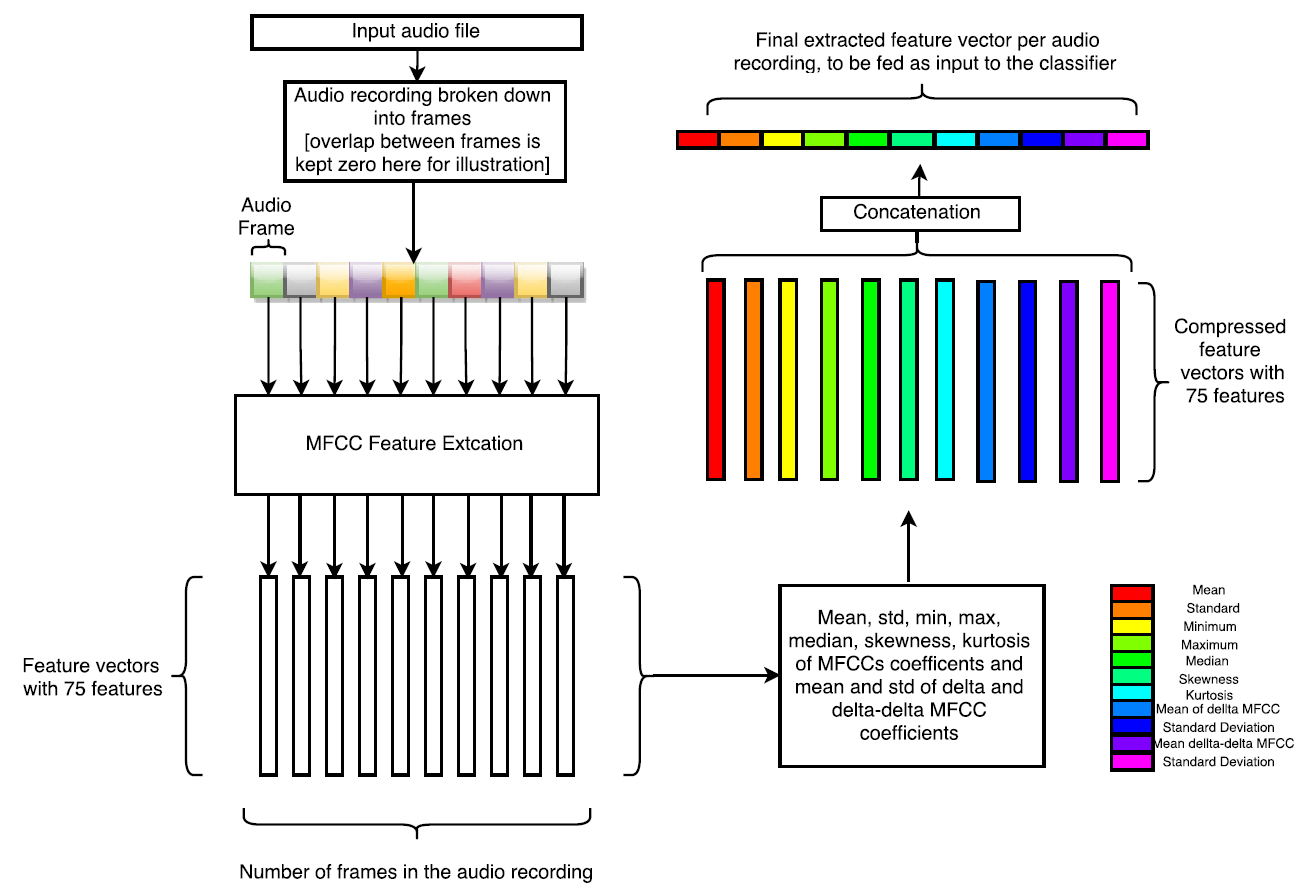
\includegraphics[width=0.95\columnwidth]{feat_extract_knn_db1}
\caption[Audio Features Extraction Schematic for kNN model]{Audio Features Extraction Schematic for kNN model}
\label{fig:feat_extract_knn_db1} 
\end{figure}

\begin{table}[tb]
\caption[Parameters for MFCC extraction]{Parameters for MFCC extraction}
\label{tab:param_mfcc_knn_db1}
\centering
\begin{tabular}{ccc}
\toprule
Parameter & Value \\
\midrule
Number of MFCC coefficients	& 25\\
Number of mel filters	& 40\\
Frame length & 23.2 (millisec)\\
Frame shift 	& 11.6(millisec)\\
Maximum allowed frequency & 22050(Hz)\\
Minimum allowed frequency & 0(Hz)\\
Windowing type & Hamming\\
Normalize mel filters (yes/no) & Yes \\
Delta MFCC context (number of neighbor frames to be included) & 21 \\
Delta-delta MFCC context & 11 \\
Channel input & 2 (channels) \\
Pre-emphasis value & 0 \\
Cepstrum lifter type & None \\
Cepstrum lifter value & 0 \\
Denoising in mel domain (yes/no) & No \\
\bottomrule 
\end{tabular}
\end{table}

\subsubsection{Classification}
We train a k-nearest neighbors classifier with $k=5$. A 10-fold cross validation experiment is run to obtain the classification performance results, where we ascertain that no two folds have audio slices/segments/excerpts from the same audio recording. The input audio feature is 275-dimensional as discussed in the previous sub-section, and the output of the classifier is a single class label, for e.g. '0' for class 'air-conditioner', '1' for 'car-horn', etc. We tried various distance measures to quantify the closeness of a data point with its neighbors, such as 'euclidean', 'cosine', 'correlation-based similarity', etc. and found that 'cosine' distance was the best distance measure in our case. Hence, we used it in obtaining the kNN results. Complete implementation of this model was performed using Matlab. The neighborhood selection method was chosen as 'exhaustive'.

\subsection{Deep Neural Network}

\subsubsection{System Overview}
Similar to the kNN model, we use spectral feature - MFCCs of the audio recordings as an input to this model. The DNN is trained with these features as input and the class labels of the audio classes as output. Posterior probabilities of audio event classes are obtained as DNN predictions. During training, the network parameters are updated to minimize a cost function C, which is a function of the posterior probabilities and target outputs. During testing, the posterior probabilities are transformed using a softmax transformation and zero-one classification error is then calculated for the testing example. Figure~\ref{fig:system_overview_db1} illustrates a high-level idea of how the system functions.

\begin{figure}[!htb] 
\centering 
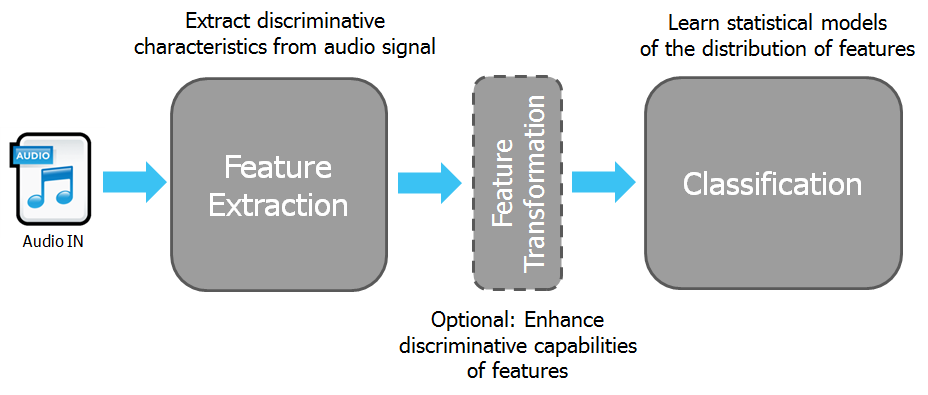
\includegraphics[width=0.95\columnwidth]{system_overview_db1}
\caption[Audio Classification Framework]{Audio Classification Framework}
\label{fig:system_overview_db1} 
\end{figure}

\subsubsection{Audio Features}
Audio features are expected to provide a reasonable representation of the time-frequency characteristics of the audio signal. MFCCs are one of the most used and successful audio features for speech recognition and events classification tasks, hence we use MFCCs as the audio features for our model. We extract the top 25 MFCC coefficients and also take the corresponding 25 delta-MFCCs and delta-delta MFCCs. This makes the input feature vector 75-dimensional. Each audio recording is broken down into constituent frames and then the mean and standard deviation of the features vectors computed over all the frames are concatenated, resulting in a vector of size 150 $(75+75=150)$. Figure~\ref{fig:feature_extraction_dnn_db1} shows the schematic for the feature extraction process. We used Sony's WriteFeat tool for extracting the MFCC features from the audio files/recordings. The parameter values used for MFCC extraction are the same as used in kNN model (see table~\ref{tab:param_mfcc_knn_db1})

\begin{figure}[!htb] 
\centering 
\includegraphics[width=0.95\columnwidth]{feature_extraction_dnn_db1}
\caption[Audio Feature Extraction Schematic - DNN]{Audio Feature Extraction Schematic - DNN}
\label{fig:feature_extraction_dnn_db1} 
\end{figure}

\subsubsection{Classification}
The neural network architecture that we developed for this dataset is inspired from \cite{gencoglu2014recognition}. There are 5 hidden layers each with 70 neurons. The final layer outputs a vector of size (10,) with the softmax probabilities for the 10 audio classes. We use sigmoid activation throughout the network, Instead of directly training the network with random initialization of the neurons, we pre-train the network using an auto-encoder pre-training technique. The details of the network architecture are presented in figure~\ref{fig:dnn_network_db1}

\begin{figure}[!htb] 
\centering 
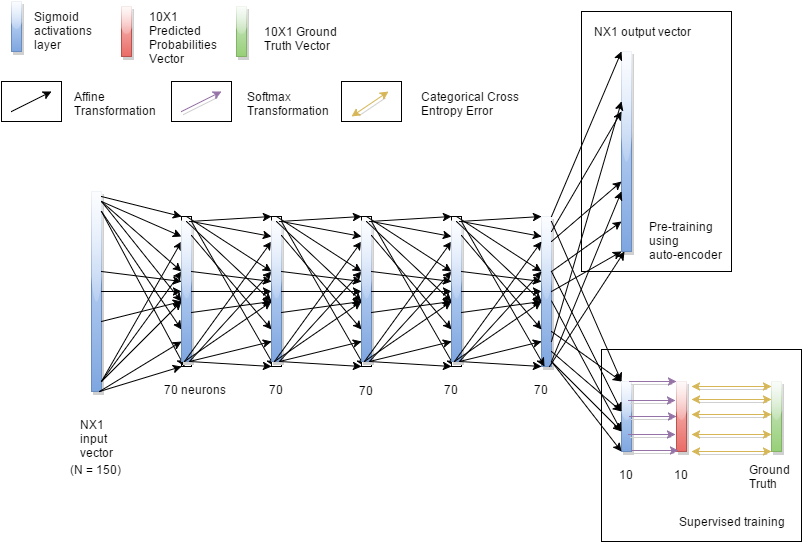
\includegraphics[width=0.95\columnwidth]{dnn_network_db1}
\caption[DNN Network Architecture]{DNN Network Architecture}
\label{fig:dnn_network_db1} 
\end{figure}

Categorical cross-entropy is used as the cost function for the training process. Zero-one error is the error-metric used for the evaluation of the performance of this classifier. The output or target audio class labels are actually one-hot vectors of size (10,). Complete implementation of the network architecture as well as the training and testing algorithm is performed using sDeePy\footnote{sDeePy provides high-level APIs on top of the basic Theano functions which makes it convenient to create, train and test neural networks.}, which is Sony's deep learning library developed in python that allows ti define, optimize and evaluate mathematical expressions involving multi-dimensional arrays efficiently.

\subsection{Convolutional Neural Network}

\subsubsection{System Overview} \label{overview_cnn_db1}
In this dataset, we have most of the audio recordings sliced into audio segments of a fixed length (4 seconds). This means that all the audio recordings consist of a constant number of frames. Hence, we can imagine an audio recording as a one dimensional image, where each pixel of this image is equivalent to each frame of the audio recording. For each frame, we also compute the MFCC features as done for the kNN and DNN models. This implies that each pixel of the image can be mapped to a feature set. In other words, the one dimensional image can be represented in terms of feature maps. This manipulation facilitates us to use a CNN model on audio data just as it is used on images.

\subsubsection{Audio Features} \label{features_cnn_db1}
As used in the above two models - kNN and DNN, we used MFCCs as the audio features for this model and extracted the top 25 MFCC coefficients along with the corresponding delta-MFCCs and delta-delta-MFCCs for each frame of each audio recording. Here, we ignore the first MFCC coefficient, as it is usually done in the literature because it just represents the log of the total energy of an audio frame, hence doesn't carry any unique or useful characteristic information. After excluding the first MFCC coefficient, we obtain an input feature vector of size (74,) per audio frame. 

A single audio frame is broken down into, say, N frames and since N is constant, each audio recording can be considered as a one-dimensional vector of size (N,). Each frame, in turn, can be represented as a feature vector of size (74,). Hence we can say that each audio recording is a one dimensional image and can be represented by 74 MFCC feature maps. By this interpretation of audio recordings, it is possible to construct a CNN architecture that takes these 74 feature maps as its input. 

We used Sony's WriteFeats tool for MFCC extraction and the parameter values used in extracting the MFCCs are the same as those used in the kNN model (see table~\ref{tab:param_mfcc_knn_db1}).

\subsubsection{Classification}
We use the CNN architecture as shown in figure~\ref{fig:cnn_db1}. There is one convolutional layer with 74 different kernels of size (3,1) that convolve over the 74 respective input feature maps to produce 10 output feature maps. This layer is followed by a pooling layer, that max-pools 1 out of the 12 convolved features providing compressed representation. Finally, we have an affine/fully-connected layer that gives an output of size (10,). A subsequent softmax transformation provides the softmax probabilities for the 10 classes. We use sigmoid activation function in all the layers, throughout the network. 

\begin{figure}[!htb] 
\centering 
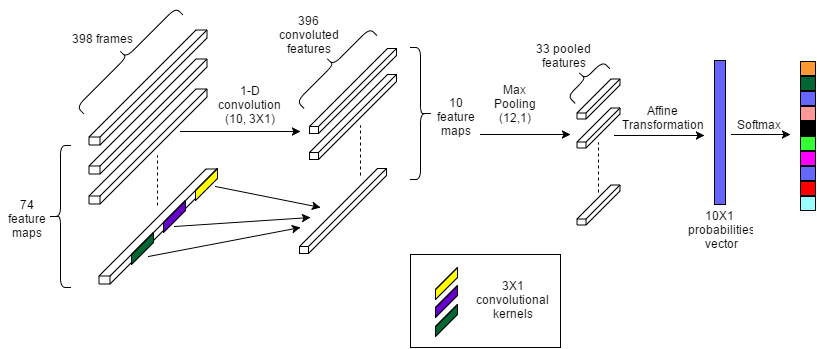
\includegraphics[width=0.95\columnwidth]{cnn_db1}
\caption[CNN Network Architecture]{CNN Network Architecture}
\label{fig:cnn_db1} 
\end{figure}

We use a learning rate of 0.0003 for training with a batch size of 50 data instances. The training is done for 1000 epochs. We do not use momentum or dropouts or any other optimization. We maintain separate training and validation data samples, with 4500 training samples and 1200 validation samples. A data sample, here, simply means an audio recording that is pre-processed into 74 feature maps.

Categorical cross-entropy is used as the cost function for the training process. Zero-one error is used as the error-metric for evaluation of the classifier performance. The output/target audio class labels are one-hot vectors of size (10,) as in the DNN model. Complete implementation of the CNN model is performed using Sony's sDeePy library.


\section{Dataset-II}
For performing the polyphonic audio event detection task on this dataset, we developed a convolutional neural network (CNN) and we also developed a support vector machine (SVM) model to reproduce the baseline results available from the literature. First we performed the classification using the SVM model, then after getting our baseline results we performed the classification task using CNN. In the following, we describe these two models. For each of the models, first we provide an overview, then discuss the audio features that were used as the input to the models, and then we describe the complete classification procedure that takes place inside these models.

\subsection{Support Vector Machine}

\subsubsection{System Overview}
An SVM model is a representation of the training examples as points in a space, mapped so that the examples of the separate categories are divided by a clear gap that is as wide as possible. New (test) examples are then mapped into that same space and predicted to belong to a category or class based on the side of the gap they fall \cite{wiki:xxx}. If the distance metric between the examples mapped as points in the classification space is linear, then the SVM performs linear classification. But, we can define other distance metrics which are not linear, making the SVM a no-linear and a more complex classifier. These distances are expressed using kernel functions. We use a radial basis function (RBF) kernel function for our SVM classifier. We developed the SVM model in order to reproduce the baseline literature results.

\subsubsection{Audio Features} \label{feats_svm}
We use MFCCs as the audio features for this model. The audio recordings are split into audio segments of 5 seconds, and for each segment we extract 25 MFCC coefficients for each audio frame within the segment. Finally, we take the mean and standard deviation of the MFCC coefficients over all the frames of a recordings. After concatenating the mean and standard deviation vectors, we get an input feature vector of size (50,) for each audio segment of 5 seconds. The schematic diagram for the feature extraction process is shown in figure~\ref{fig:feature_extraction_svm_db2}. We used Sony's WriteFeats tool for extracting the MFCC coefficients from the audio recordings. The parameter setting used in extracting the MFCC coefficients are shown in table~\ref{tab:param_mfcc_svm_db2}. Mos of these settings are derived from \cite{kons2013audio}.

\begin{figure}[!htb] 
\centering 
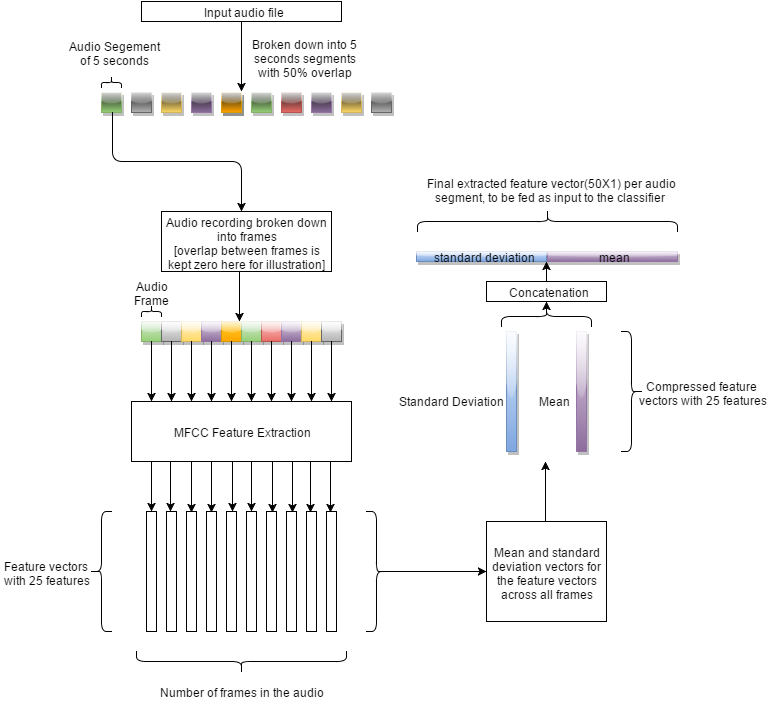
\includegraphics[width=0.95\columnwidth]{feature_extraction_svm_db2}
\caption[Feature Extraction Schematic for SVM model]{Feature Extraction Schematic for SVM model}
\label{fig:feature_extraction_svm_db2} 
\end{figure}

\begin{table}[tb]
\caption[Parameters for MFCC extraction for SVM for dataset-II]{Parameters for MFCC extraction dataset-II}
\label{tab:param_mfcc_svm_db2}
\centering
\begin{tabular}{ccc}
\toprule
Parameter & Value \\
\midrule
Number of MFCC coefficients	& 25\\
Number of mel filters	& 30\\
Frame length & 46 (millisec)\\
Frame shift 	& 23 (millisec)\\
Maximum allowed frequency & 7500 (Hz)\\
Minimum allowed frequency & 80 (Hz)\\
Windowing type & Hamming\\
Normalize mel filters (yes/no) & Yes \\
Channel input & 2 (channels) \\
\bottomrule 
\end{tabular}
\end{table}

\subsubsection{Classification}
Following the approach used in \cite{kons2013audio}, we used an RBF kernel function (with $\gamma = 0.2$). An RBF kernel function on two samples x and x', represented as feature vectors, is defined as:

\begin{eqnarray*}
K(x,x') = w^{-\frac{{\|x-x'\|}^2}{2\sigma^2}}
\end{eqnarray*}

For other parameters, we used the values used in \cite{kons2013audio}. We trained 4 binary SVM classifiers for the 4 classes, by taking all the training data belonging to that class as positive examples and the rest of the data as negative examples. We normalized the input features to the range [0,1] with the scaling estimated from training data being applied to the test data. Matlab was used for implementing the SVM model.

\subsection{Convolutional Neural Network}

\subsubsection{System Overview}
As discussed in section \ref{feats_svm}, the audio recordings obtained from \cite{kons2013audio} are segmented into recordings of a fixed duration - 5 seconds, with 50\% overlap. This implies that all the audio recordings have the same number of constituent audio frames. Hence, we can imagine each audio recording as a 1-dimensional image (as explained in sections~\ref{overview_cnn_db1} and \ref{features_cnn_db1}). We then extract MFCC coefficients out of each audio frame as a part of the feature extraction step. These MFCC features of each audio frame can be considered as the features maps for the whole audio recording. Finally, the audio recording, which is now represented by these feature maps can be fed as input to the convolutional neural network.

\subsubsection{Audio Features}
As stated in the previous section, we use MFCCs as the audio features for this model. We extract 25 MFCC coefficients for each audio frame of each audio recording. The first MFCC coefficient is ignored as it is the log of the total energy of a frame, hence, doesn't provide any discriminatory information. Thus, we get an input feature vector of size (24,) per audio frame.

Now, each audio recording is broken down into say \textsl{M} segments, each segment of 5 seconds. Each of the \textsl{M} segments is then broken down into \textsl{N} frames, and since \textsl{N} is constant, each audio segment can be considered as a 1-dimensional image represented as 24 MFCC feature maps (see section\ref{features_cnn_db1} for a detailed explanation). We used Sony's WriteFeats tool for extracting the MFCCs from the audio recordings, and the parameter values used for the extraction are specified under table~\ref{tab:param_mfcc_cnn_db2}. By using these parameter values, we generate 215 frames for each audio recording.

\begin{table}[tb]
\caption[Parameters for MFCC extraction for CNN for dataset-II]{Parameters for MFCC extraction for CNN  for dataset-II}
\label{tab:param_mfcc_cnn_db2}
\centering
\begin{tabular}{ccc}
\toprule
Parameter & Value \\
\midrule
Number of MFCC coefficients	& 25\\
Number of mel filters	& 30\\
Frame length & 30 (millisec)\\
Frame shift 	& 10 (millisec)\\
Maximum allowed frequency & 11025 (Hz)\\
Minimum allowed frequency & 0 (Hz)\\
Windowing type & Hamming\\
Normalize mel filters (yes/no) & Yes \\
Channel input & 2 (channels) \\
\bottomrule 
\end{tabular}
\end{table}

\subsubsection{Classification}
The convolutional neural network architecture is shown in figure~\ref{fig:cnn_model_db2}. There is 1 convolutional layer with 24 kernels of size (8,1) that convolve over the 24 respective feature maps to produce 4 output feature maps. This layer is followed by a pooling layer, that max-pools 1 out of the 16 convolved features resulting in a compressed representation. Subsequently, there is an affine/fully-connected layer that provides a single unit output from the 4 compressed feature maps. Finally, there is a sigmoid transformation over the single unit output that gives us the predicted probability of the binary classifier. We use tanh activation function for the hidden layers of the network. THe network consists of 768 convolutional layer paramters and 54 fully connected parameters summing to a total of 820 parameters.

We find the learning rate of 0.003, and a batch size of 50 suitable for the classification task. The training is done for 1000 epochs. We do not use momentum, dropouts or any other such optimization. We roughly have 3500 training and 800 validation data samples. Here, each data sample refers to an audio segment which is pre-processed into MFCC features.

Weighted binary cross-entropy is used as the cost-function for the training process. Different classes are assigned different weights such that the weights are inversely proportional to the size of each class. These weights are then used as an extra parameter inside the standard cross entropy function to account for the skew in the proportion of the positive and negative samples of the classifier (details discussed in the results section). For the evaluation of the classifier performance, equal error rate is used as the error metric. The choice of these error metrics for the cost function and for the evaluation is motivated from \cite{kons2013audio}. The CNN architecture as well as the training and evaluation procedures are implemented using Sony's deep learning library - sDeePy.

\begin{figure}[!htb] 
\centering 
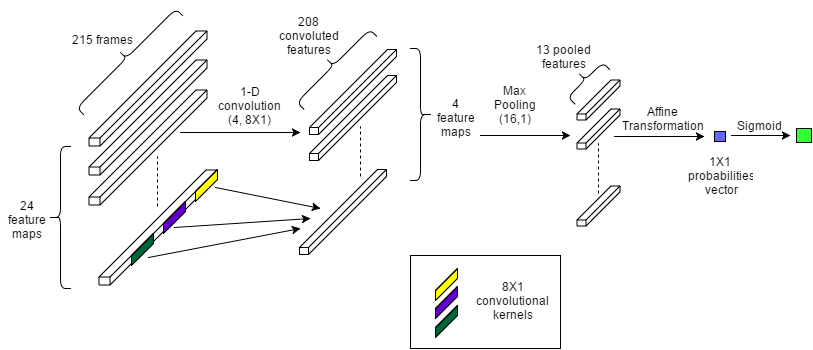
\includegraphics[width=0.95\columnwidth]{cnn_model_db2}
\caption[CNN model architecture for dataset-II]{[CNN model architecture for dataset-II}
\label{fig:cnn_model_db2} 
\end{figure}


\section{Dataset-III}
For this dataset, we developed two models. First we implemented a Gaussian Mixture Model (GMM) to reproduce the baseline results for this dataset published in \cite{foster2015chime}. Then we implemented our own Convolutional Neural Network (CNN) which was motivated from the experience of implementing CNNs for dataset-I and dataset-II. In the following we describe these two models.

\subsection{Gaussian Mixture Model}

\subsubsection{System Overview}
To reproduce the baseline GMM results of \cite{foster2015chime}, we implemented a similar GMM model. We extracted MFCC features out of the audio recordings and estimated GMMs on sequences of the MFCC features. GMM is often used in combination with MFCC features in the literature for tackling speech recognition or sound classification systems (\cite{stowelldetection}, \cite{defreville2006automatic}, \cite{aucouturier2007bag}).

\subsubsection{Audio Features}
The parameters for the extraction of MFCC features are derived from \cite{foster2015chime}. The parameter setting used in MFCC extraction from the audio recordings is shown in table~\ref{tab:param_mfcc_db3}. After discarding the first MFCC coefficient (which represents the frame energy), we get 13 MFCCs for each audio frame for each audio recording for estimating the GMMs. Complete feature extraction process is performed using Sony's WriteFeat tool.

\subsubsection{Classification}
For each of the 7 audio classes of the dataset, we estimate a pair of GMMs (as done in \cite{foster2015chime}). Using the expectation-maximization algorithm, we estimate full-covariance Gaussians. The number of Gaussians in the GMMs are varied as the values in the set: {1,2,4,8}. For predicting the presence or absence of an audio class, we calculate the log-likelihood ratio of the associated 

\begin{table}[tb]
\caption[Parameters for MFCC extraction for dataset-III]{Parameters for MFCC extraction for dataset-III}
\label{tab:param_mfcc_db3}
\centering
\begin{tabular}{ccc}
\toprule
Parameter & Value \\
\midrule
Number of MFCC coefficients	& 25\\
Number of mel filters	& 30\\
Frame length & 46 (millisec)\\
Frame shift 	& 23 (millisec)\\
Maximum allowed frequency & 7500 (Hz)\\
Minimum allowed frequency & 80 (Hz)\\
Windowing type & Hamming\\
Normalize mel filters (yes/no) & Yes \\
Channel input & 2 (channels) \\
\bottomrule 
\end{tabular}
\end{table}